% Options for packages loaded elsewhere
\PassOptionsToPackage{unicode}{hyperref}
\PassOptionsToPackage{hyphens}{url}
%
\documentclass[
]{report}
\usepackage{amsmath,amssymb}
\usepackage{iftex}
\ifPDFTeX
  \usepackage[T1]{fontenc}
  \usepackage[utf8]{inputenc}
  \usepackage{textcomp} % provide euro and other symbols
\else % if luatex or xetex
  \usepackage{unicode-math} % this also loads fontspec
  \defaultfontfeatures{Scale=MatchLowercase}
  \defaultfontfeatures[\rmfamily]{Ligatures=TeX,Scale=1}
\fi
\usepackage{lmodern}
\ifPDFTeX\else
  % xetex/luatex font selection
\fi
% Use upquote if available, for straight quotes in verbatim environments
\IfFileExists{upquote.sty}{\usepackage{upquote}}{}
\IfFileExists{microtype.sty}{% use microtype if available
  \usepackage[]{microtype}
  \UseMicrotypeSet[protrusion]{basicmath} % disable protrusion for tt fonts
}{}
\makeatletter
\@ifundefined{KOMAClassName}{% if non-KOMA class
  \IfFileExists{parskip.sty}{%
    \usepackage{parskip}
  }{% else
    \setlength{\parindent}{0pt}
    \setlength{\parskip}{6pt plus 2pt minus 1pt}}
}{% if KOMA class
  \KOMAoptions{parskip=half}}
\makeatother
\usepackage{xcolor}
\usepackage{color}
\usepackage{fancyvrb}
\newcommand{\VerbBar}{|}
\newcommand{\VERB}{\Verb[commandchars=\\\{\}]}
\DefineVerbatimEnvironment{Highlighting}{Verbatim}{commandchars=\\\{\}}
% Add ',fontsize=\small' for more characters per line
\usepackage{framed}
\definecolor{shadecolor}{RGB}{248,248,248}
\newenvironment{Shaded}{\begin{snugshade}}{\end{snugshade}}
\newcommand{\AlertTok}[1]{\textcolor[rgb]{0.94,0.16,0.16}{#1}}
\newcommand{\AnnotationTok}[1]{\textcolor[rgb]{0.56,0.35,0.01}{\textbf{\textit{#1}}}}
\newcommand{\AttributeTok}[1]{\textcolor[rgb]{0.13,0.29,0.53}{#1}}
\newcommand{\BaseNTok}[1]{\textcolor[rgb]{0.00,0.00,0.81}{#1}}
\newcommand{\BuiltInTok}[1]{#1}
\newcommand{\CharTok}[1]{\textcolor[rgb]{0.31,0.60,0.02}{#1}}
\newcommand{\CommentTok}[1]{\textcolor[rgb]{0.56,0.35,0.01}{\textit{#1}}}
\newcommand{\CommentVarTok}[1]{\textcolor[rgb]{0.56,0.35,0.01}{\textbf{\textit{#1}}}}
\newcommand{\ConstantTok}[1]{\textcolor[rgb]{0.56,0.35,0.01}{#1}}
\newcommand{\ControlFlowTok}[1]{\textcolor[rgb]{0.13,0.29,0.53}{\textbf{#1}}}
\newcommand{\DataTypeTok}[1]{\textcolor[rgb]{0.13,0.29,0.53}{#1}}
\newcommand{\DecValTok}[1]{\textcolor[rgb]{0.00,0.00,0.81}{#1}}
\newcommand{\DocumentationTok}[1]{\textcolor[rgb]{0.56,0.35,0.01}{\textbf{\textit{#1}}}}
\newcommand{\ErrorTok}[1]{\textcolor[rgb]{0.64,0.00,0.00}{\textbf{#1}}}
\newcommand{\ExtensionTok}[1]{#1}
\newcommand{\FloatTok}[1]{\textcolor[rgb]{0.00,0.00,0.81}{#1}}
\newcommand{\FunctionTok}[1]{\textcolor[rgb]{0.13,0.29,0.53}{\textbf{#1}}}
\newcommand{\ImportTok}[1]{#1}
\newcommand{\InformationTok}[1]{\textcolor[rgb]{0.56,0.35,0.01}{\textbf{\textit{#1}}}}
\newcommand{\KeywordTok}[1]{\textcolor[rgb]{0.13,0.29,0.53}{\textbf{#1}}}
\newcommand{\NormalTok}[1]{#1}
\newcommand{\OperatorTok}[1]{\textcolor[rgb]{0.81,0.36,0.00}{\textbf{#1}}}
\newcommand{\OtherTok}[1]{\textcolor[rgb]{0.56,0.35,0.01}{#1}}
\newcommand{\PreprocessorTok}[1]{\textcolor[rgb]{0.56,0.35,0.01}{\textit{#1}}}
\newcommand{\RegionMarkerTok}[1]{#1}
\newcommand{\SpecialCharTok}[1]{\textcolor[rgb]{0.81,0.36,0.00}{\textbf{#1}}}
\newcommand{\SpecialStringTok}[1]{\textcolor[rgb]{0.31,0.60,0.02}{#1}}
\newcommand{\StringTok}[1]{\textcolor[rgb]{0.31,0.60,0.02}{#1}}
\newcommand{\VariableTok}[1]{\textcolor[rgb]{0.00,0.00,0.00}{#1}}
\newcommand{\VerbatimStringTok}[1]{\textcolor[rgb]{0.31,0.60,0.02}{#1}}
\newcommand{\WarningTok}[1]{\textcolor[rgb]{0.56,0.35,0.01}{\textbf{\textit{#1}}}}
\usepackage{longtable,booktabs,array}
\usepackage{calc} % for calculating minipage widths
% Correct order of tables after \paragraph or \subparagraph
\usepackage{etoolbox}
\makeatletter
\patchcmd\longtable{\par}{\if@noskipsec\mbox{}\fi\par}{}{}
\makeatother
% Allow footnotes in longtable head/foot
\IfFileExists{footnotehyper.sty}{\usepackage{footnotehyper}}{\usepackage{footnote}}
\makesavenoteenv{longtable}
\usepackage{graphicx}
\makeatletter
\def\maxwidth{\ifdim\Gin@nat@width>\linewidth\linewidth\else\Gin@nat@width\fi}
\def\maxheight{\ifdim\Gin@nat@height>\textheight\textheight\else\Gin@nat@height\fi}
\makeatother
% Scale images if necessary, so that they will not overflow the page
% margins by default, and it is still possible to overwrite the defaults
% using explicit options in \includegraphics[width, height, ...]{}
\setkeys{Gin}{width=\maxwidth,height=\maxheight,keepaspectratio}
% Set default figure placement to htbp
\makeatletter
\def\fps@figure{htbp}
\makeatother
\setlength{\emergencystretch}{3em} % prevent overfull lines
\providecommand{\tightlist}{%
  \setlength{\itemsep}{0pt}\setlength{\parskip}{0pt}}
\setcounter{secnumdepth}{5}
% definitions for citeproc citations
\NewDocumentCommand\citeproctext{}{}
\NewDocumentCommand\citeproc{mm}{%
  \begingroup\def\citeproctext{#2}\cite{#1}\endgroup}
\makeatletter
 % allow citations to break across lines
 \let\@cite@ofmt\@firstofone
 % avoid brackets around text for \cite:
 \def\@biblabel#1{}
 \def\@cite#1#2{{#1\if@tempswa , #2\fi}}
\makeatother
\newlength{\cslhangindent}
\setlength{\cslhangindent}{1.5em}
\newlength{\csllabelwidth}
\setlength{\csllabelwidth}{3em}
\newenvironment{CSLReferences}[2] % #1 hanging-indent, #2 entry-spacing
 {\begin{list}{}{%
  \setlength{\itemindent}{0pt}
  \setlength{\leftmargin}{0pt}
  \setlength{\parsep}{0pt}
  % turn on hanging indent if param 1 is 1
  \ifodd #1
   \setlength{\leftmargin}{\cslhangindent}
   \setlength{\itemindent}{-1\cslhangindent}
  \fi
  % set entry spacing
  \setlength{\itemsep}{#2\baselineskip}}}
 {\end{list}}
\usepackage{calc}
\newcommand{\CSLBlock}[1]{\hfill\break\parbox[t]{\linewidth}{\strut\ignorespaces#1\strut}}
\newcommand{\CSLLeftMargin}[1]{\parbox[t]{\csllabelwidth}{\strut#1\strut}}
\newcommand{\CSLRightInline}[1]{\parbox[t]{\linewidth - \csllabelwidth}{\strut#1\strut}}
\newcommand{\CSLIndent}[1]{\hspace{\cslhangindent}#1}
\usepackage{booktabs}
\usepackage{geometry}
\usepackage[none]{hyphenat}
\usepackage{titlesec}
\usepackage{longtable}
\usepackage{xcolor}
\usepackage{setspace}
\usepackage{pdfpages}

\pagestyle{plain}

%%%% Set margins
\setlength{\topmargin}{-1cm}
\addtolength{\evensidemargin}{-1cm}
\addtolength{\oddsidemargin}{-1cm}
\addtolength{\textheight}{3cm}
\addtolength{\textwidth}{2cm}

% Spacing for reading guides
\newcommand{\rgs}{\vspace{12pt}} % Vertical space
\newcommand{\rgi}{\hspace{24pt}}  % Indent

\newcommand\latexcode[1]{#1}

% Format chapter titles and spacing
\renewcommand*{\chaptername}{Module}

\titleformat{\chapter}[display]
{\bfseries\Large}
{\filleft\MakeUppercase{\chaptertitlename} \Huge\thechapter}
{3ex}
{\titlerule
\vspace{1.5ex}%
\filright}
[\vspace{1.5ex}%
\titlerule]
\titlespacing*{\chapter}{0pt}{-40pt}{20pt}
\ifLuaTeX
  \usepackage{selnolig}  % disable illegal ligatures
\fi
\usepackage{bookmark}
\IfFileExists{xurl.sty}{\usepackage{xurl}}{} % add URL line breaks if available
\urlstyle{same}
\hypersetup{
  hidelinks,
  pdfcreator={LaTeX via pandoc}}

\title{\textbf{STAT 216 Coursepack}\\
\strut \\
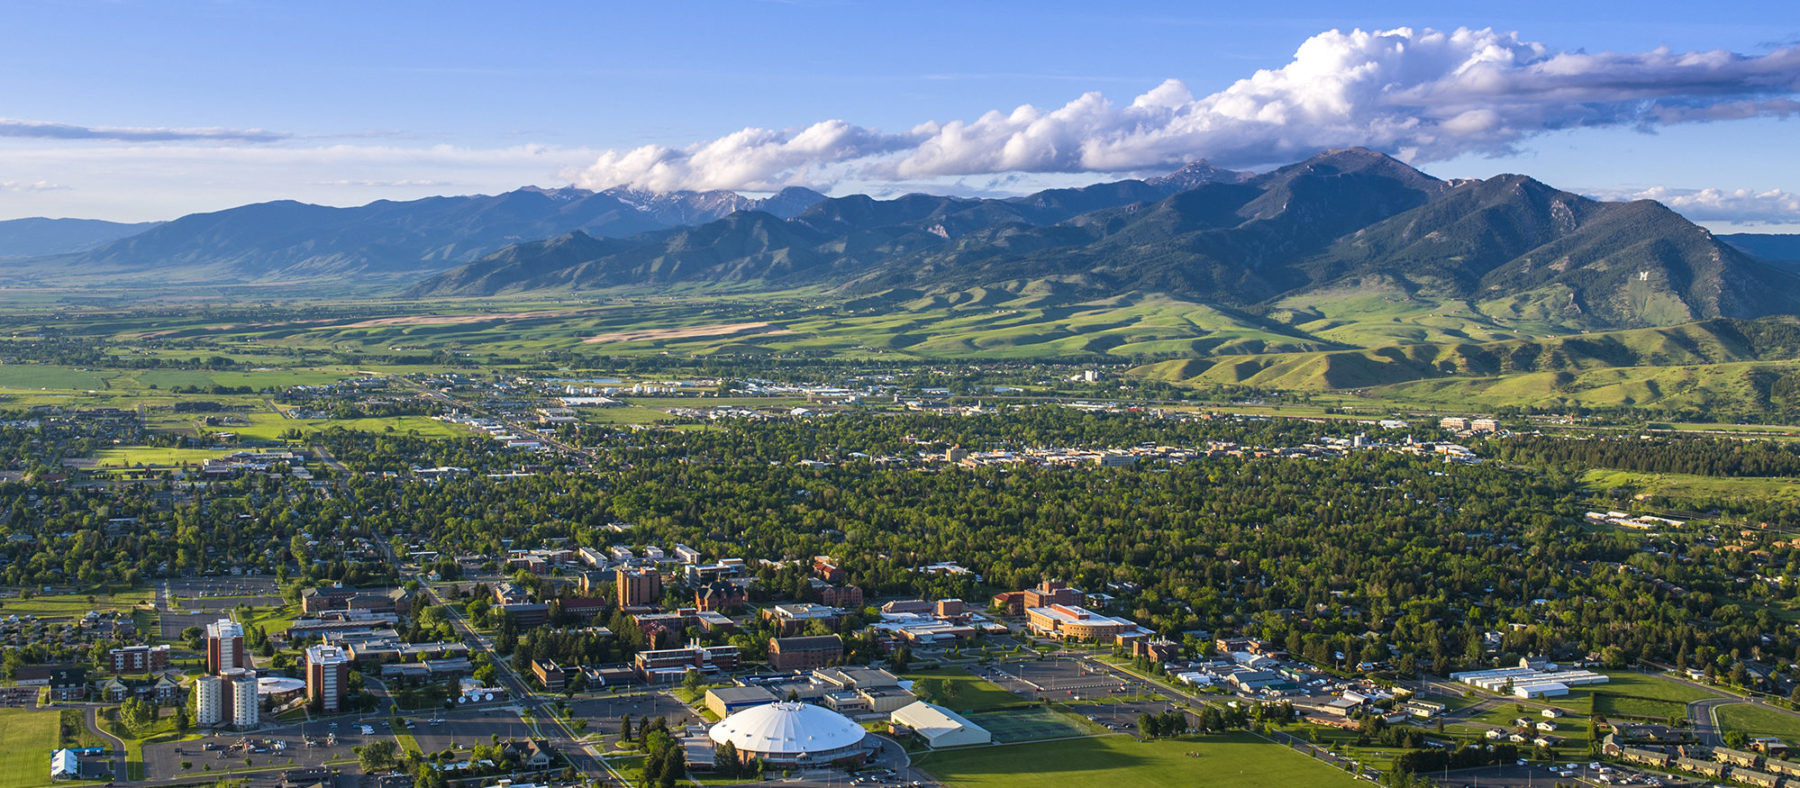
\includegraphics[width=5in,height=\textheight]{images/msu-campus.jpg}}
\usepackage{etoolbox}
\makeatletter
\providecommand{\subtitle}[1]{% add subtitle to \maketitle
  \apptocmd{\@title}{\par {\large #1 \par}}{}{}
}
\makeatother
\subtitle{Spring 2025\\
Montana State University}
\author{Melinda Yager\\
Jade Schmidt\\
Stacey Hancock}
\date{}

\begin{document}
\maketitle

\newpage
\thispagestyle{empty}

This resource was developed by Melinda Yager, Jade Schmidt, and Stacey Hancock in 2021 to accompany the online textbook: Hancock, S., Carnegie, N., Meyer, E., Schmidt, J., and Yager, M. (2021). \emph{Montana State Introductory Statistics with R}. Montana State University. \url{https://mtstateintrostats.github.io/IntroStatTextbook/}.

This resource is released under a \href{https://creativecommons.org/licenses/by-nc-sa/4.0/}{Creative Commons BY-NC-SA 4.0} license unless otherwise noted.

\setcounter{tocdepth}{1}
\addtocontents{toc}{\protect\thispagestyle{empty}}
\tableofcontents
\thispagestyle{empty}

\newpage
\setcounter{page}{1}

\chapter*{Preface}\label{preface}
\addcontentsline{toc}{chapter}{Preface}

This coursepack accompanies the textbook for STAT 216: Montana State Introductory Statistics with R, which can be found at \url{https://mtstateintrostats.github.io/IntroStatTextbook/}. The syllabus for the course (including the course calendar), data sets, and links to D2L Brightspace, Gradescope, and the MSU RStudio server can be found on the course webpage: \url{https://math.montana.edu/courses/s216/}.
Other notes and review materials are linked in D2L.

Each of the activities in this workbook is designed to target specific learning outcomes of the course, giving you practice with important statistical concepts in a group setting with instructor guidance. In addition to the in-class activities for the course, video notes are provided to aid in taking notes while you complete the required videos. Bring this workbook with you to class each class period, and take notes in the workbook as you would your own notes. A well-written completed workbook will provide an optimal study guide for exams!

All activities and labs in this coursepack will be completed during class time. Parts of each lab will be turned in on Gradescope. To aid in your understanding, read through the introduction for each activity before attending class each day.

STAT 216 is a 3-credit in-person course. In our experience, it takes six to nine hours per week outside of class to achieve a good grade in this class. By ``good'' we mean at least a C because a grade of D or below does not count toward fulfilling degree requirements. Many of you set your goals higher than just getting a C, and we fully support that. You need roughly nine hours per week to review past activities, read feedback on previous assignments, complete current assignments, and prepare for the next day's class. A typical week in the life of a STAT 216 student looks like:

\begin{itemize}
\tightlist
\item
  \emph{Prior to class meeting}:

  \begin{itemize}
  \tightlist
  \item
    Read assigned sections of the textbook, using the provided reading guides to take notes on the material.
  \item
    Watch the provided videos, taking notes in the coursepack.
  \item
    Read through the introduction to the day's in-class activity.
  \item
    Read through the week's homework assignment and note any questions you may have on the content.
  \end{itemize}
\item
  \emph{During class meeting}:

  \begin{itemize}
  \tightlist
  \item
    Work through the guided activity, in-class activity or weekly lab with your classmates and instructor, taking detailed notes on your answers to each question in the activity.
  \end{itemize}
\item
  \emph{After class meeting}:

  \begin{itemize}
  \tightlist
  \item
    Complete any parts of the activity you did not complete in class.
  \item
    Review the activity solutions in the Math and Stat Center, and take notes on key points.
  \item
    Complete any remaining assigned readings for the week.
  \item
    Complete the week's homework assignment.
  \end{itemize}
\end{itemize}

\nocite{*}

\chapter{Unit 1 Review}\label{unit-1-review}

The following module contains both a list of key topics covered in Unit 1 as well as Module Review Worksheets that will be covered in Weekly Review Sessions.

\section{Module Review}\label{module-review}

\setstretch{1}

The following worksheets review each of the modules. These worksheets will be completed during Melinda's Study Sessions each week. Solutions will be posted on D2L in the Unit 1 Review folder after the study sessions.

\section{Key Topics}\label{key-topics}

Review the key topics for Unit 1 prior to the first exams. All of these topics will be covered in Modules 1--4.

\newpage

\section{Module 1 Review - Sampling Methods}\label{module-1-review---sampling-methods}

\begin{enumerate}
\def\labelenumi{\arabic{enumi}.}
\tightlist
\item
  Suppose that the proportion of all American adults that fit the medical definition of being obese is 0.23. A large medical clinic would like to determine if the proportion of their patients that are obese is higher than that of all American adults. The clinic takes a simple random sample of 30 of their patients and finds that 9 patients in the sample are obese.
\end{enumerate}

\begin{enumerate}
\def\labelenumi{\alph{enumi}.}
\tightlist
\item
  What is the target population?
\end{enumerate}

\vspace{0.4in}

\begin{enumerate}
\def\labelenumi{\alph{enumi}.}
\setcounter{enumi}{1}
\tightlist
\item
  What are the observational units?
\end{enumerate}

\vspace{0.4in}

\begin{enumerate}
\def\labelenumi{\alph{enumi}.}
\setcounter{enumi}{2}
\tightlist
\item
  What variable is being studied?
\end{enumerate}

\vspace{0.4in}

\begin{enumerate}
\def\labelenumi{\alph{enumi}.}
\setcounter{enumi}{3}
\tightlist
\item
  Is the variable identified in part (c) categorical or quantitative?
\end{enumerate}

\vspace{0.4in}

\begin{enumerate}
\def\labelenumi{\arabic{enumi}.}
\setcounter{enumi}{1}
\tightlist
\item
  Martha works in Macy's advertising department. She is interested in the shopping experience of all Macy's shoppers in the U.S. Every Saturday morning for a month she stands outside of the Bozeman Macy's asking people about their experience. One of the questions she uses is: ``As a huge fan of Macy's, I believe Macy's has the best choices of clothing in Bozeman. Don't you agree?'' Every person that was asked, responded.
\end{enumerate}

\begin{enumerate}
\def\labelenumi{\alph{enumi}.}
\tightlist
\item
  Identify the target population.
\end{enumerate}

\vspace{0.4in}

\begin{enumerate}
\def\labelenumi{\alph{enumi}.}
\setcounter{enumi}{1}
\tightlist
\item
  Identify the sample.
\end{enumerate}

\vspace{0.4in}

\begin{enumerate}
\def\labelenumi{\alph{enumi}.}
\setcounter{enumi}{2}
\tightlist
\item
  Which of the three types of sampling bias (selection, non-response, response) may be present? Explain your choice(s).
\end{enumerate}

\vspace{0.5in}

\newpage

\begin{enumerate}
\def\labelenumi{\arabic{enumi}.}
\setcounter{enumi}{2}
\tightlist
\item
  This study aims to explore whether Swiss university students feeling academic study pressure (whether the student had experienced academic failure) tend to use psychotropic drugs (whether the student had used psychotropic drugs during the student's time at university) as a coping mechanism. An invitation email was sent to all bachelor's and master's students at the University of Lausanne, totaling 15,400 individuals, with a link to access the online questionnaire containing 49 questions and 107 items. No reminder was sent out, and no incentive was given to complete the questionnaire. A total of 1,690 students initially participated in the study, but 424 questionnaires were too incomplete to be used for analysis and were excluded. Additionally, 67 questionnaires were removed because of significant missing sociodemographic information, resulting in 1,199 completed responses included in the final analysis. Is there an association between study pressure and use of psychotropic drugs among Swiss University students?
\end{enumerate}

\begin{enumerate}
\def\labelenumi{\alph{enumi}.}
\tightlist
\item
  Identify the target population.
\end{enumerate}

\vspace{0.4in}

\begin{enumerate}
\def\labelenumi{\alph{enumi}.}
\setcounter{enumi}{1}
\tightlist
\item
  Identify the sample.
\end{enumerate}

\vspace{0.4in}

\begin{enumerate}
\def\labelenumi{\alph{enumi}.}
\setcounter{enumi}{2}
\tightlist
\item
  Which of the three types of sampling bias (selection, non-response, response) may be present? Explain your choice(s).
\end{enumerate}

\vspace{0.5in}

\begin{enumerate}
\def\labelenumi{\alph{enumi}.}
\setcounter{enumi}{3}
\tightlist
\item
  Identify the type and roles of each variable in the study.
\end{enumerate}

\vspace{1in}

\begin{enumerate}
\def\labelenumi{\arabic{enumi}.}
\setcounter{enumi}{3}
\tightlist
\item
  Researchers decided to investigate whether a cat's coat color is associated with aggressive cat behavior by creating a 20-minute survey. The survey was distributed by posting it to social media and through cat-related listservs (e.g., For the Love of Cats), inviting individuals to take the survey. A total of 1,365 surveys were completed by participants. The frequency of each of the following aggressive behavior categories was assessed: hiss, stalk/chase, bite, slap/scratch. Frequency of behaviors toward people were recorded on a 6-point scale: 0 = never, 1 = less than once every 6 months, 2 = once every 6 months, 3 = once per month, 4 = once per week, 5 = one or more times per day. Because there were four aggressive behavior categories, each with a frequency of 0 to 5 possible, each cat could score between 0 to 20 for human aggression. Is there an association between coat color and aggressive behavior among cats?
\end{enumerate}

\begin{enumerate}
\def\labelenumi{\alph{enumi}.}
\tightlist
\item
  Identify the target population.
\end{enumerate}

\vspace{0.4in}

\begin{enumerate}
\def\labelenumi{\alph{enumi}.}
\setcounter{enumi}{1}
\tightlist
\item
  Identify the sample.
\end{enumerate}

\vspace{0.4in}

\begin{enumerate}
\def\labelenumi{\alph{enumi}.}
\setcounter{enumi}{2}
\tightlist
\item
  Which of the three types of sampling bias (selection, non-response, response) may be present? Explain your choice(s).
\end{enumerate}

\vspace{0.5in}

\begin{enumerate}
\def\labelenumi{\alph{enumi}.}
\setcounter{enumi}{3}
\tightlist
\item
  Identify the type and roles of each variable in the study.
\end{enumerate}

\vspace{1in}

\newpage

\section{Module 2 Review}\label{module-2-review}

\begin{enumerate}
\def\labelenumi{\arabic{enumi}.}
\tightlist
\item
  Spelling errors in a text can either be non-word errors (teh instead of the) or word errors (lose instead of loose). It was found that non-word errors make up about 25\% of all errors. A human proofreader will catch 92\% of non-word errors and 75\% of word errors.
\end{enumerate}

Let N represent non-word errors and C represent that a human proofreader will catch the error.

\begin{enumerate}
\def\labelenumi{\alph{enumi}.}
\item
  Identify the following values with appropriate probability notation.
  \vspace{2mm}

  \(0.25\)
  \vspace{2mm}

  \(0.92\)
  \vspace{2mm}

  \(0.75\)
  \vspace{2mm}
\item
  Fill in the table below to represent the situation:
\end{enumerate}

\begin{center}
\begin{tabular}{|c|c|c|c|} \hline
\hspace{0.8in} & \hspace{0.25in}  $N$ \hspace{.25in} & \hspace{0.25in} $N^C$ \hspace{0.25in} & \hspace{0.25in} Total \hspace{0.25in} \\ \hline
 $C$ &  &  &  \\ \hline
 $C^C$ &  & &  \\ \hline
Total &  &  & 100000 \\ \hline
\end{tabular}
\end{center}
\vspace{.1in}

\begin{enumerate}
\def\labelenumi{\alph{enumi}.}
\setcounter{enumi}{2}
\tightlist
\item
  Using your table calculate the probability that a randomly selected error caught by a human proofreader is a non-word error. Use appropriate probability notation.
\end{enumerate}

\vspace{1in}

\begin{enumerate}
\def\labelenumi{\alph{enumi}.}
\setcounter{enumi}{3}
\tightlist
\item
  Find the probability a selected error is a non-word error and was not caught by a human proofreader. Use appropriate probability notation.
\end{enumerate}

\vspace{1in}

\begin{enumerate}
\def\labelenumi{\alph{enumi}.}
\setcounter{enumi}{4}
\tightlist
\item
  Find the value of \(P(N|C)\). What does this probability mean?
\end{enumerate}

\vspace{1in}

\newpage

\begin{enumerate}
\def\labelenumi{\arabic{enumi}.}
\setcounter{enumi}{1}
\tightlist
\item
  A private college report contains these statistics:
\end{enumerate}

\begin{itemize}
\item
  70\% of incoming freshmen attended public schools
\item
  75\% of public-school students who enroll as freshmen eventually graduate
\item
  90\% of other freshmen eventually graduate
\end{itemize}

Let A represent the event that a freshman attended public school and B the event that a freshman eventually graduates.

\begin{enumerate}
\def\labelenumi{\alph{enumi}.}
\item
  Identify the following values with appropriate probability notation.
  \vspace{2mm}

  \(0.70\)
  \vspace{2mm}

  \(0.75\)
  \vspace{2mm}

  \(0.90\)
  \vspace{2mm}
\item
  Fill in the table below to represent the situation:
\end{enumerate}

\begin{center}
\begin{tabular}{|c|c|c|c|} \hline
\hspace{0.8in} & \hspace{0.25in}  $A$ \hspace{.25in} & \hspace{0.25in} $A^C$ \hspace{0.25in} & \hspace{0.25in} Total \hspace{0.25in} \\ \hline
 $B$ &  &  &  \\ \hline
 $B^C$ &  & &  \\ \hline
Total &  &  & 100000 \\ \hline
\end{tabular}
\end{center}
\vspace{.1in}

\begin{enumerate}
\def\labelenumi{\alph{enumi}.}
\setcounter{enumi}{2}
\tightlist
\item
  Calculate the probability a selected freshman attended public school given they did not graduate. Use appropriate probability notation.
\end{enumerate}

\vspace{1in}

\begin{enumerate}
\def\labelenumi{\alph{enumi}.}
\setcounter{enumi}{3}
\tightlist
\item
  Calculate the probability a selected freshman does not graduate. Use appropriate probability notation.
\end{enumerate}

\vspace{1in}

\begin{enumerate}
\def\labelenumi{\alph{enumi}.}
\setcounter{enumi}{4}
\tightlist
\item
  Of the population of freshman that attended public school, what is the probability they do not graduate. Use appropriate probability notation.
\end{enumerate}

\vspace{1in}

\begin{enumerate}
\def\labelenumi{\alph{enumi}.}
\setcounter{enumi}{5}
\tightlist
\item
  Find the value of \(P(A~\text{and}~B^C)\). Write this probability in context of the problem.
\end{enumerate}

\newpage

\section{Module 3 Review - Simulation Methods}\label{module-3-review---simulation-methods}

\begin{Shaded}
\begin{Highlighting}[]
\NormalTok{hearing }\OtherTok{\textless{}{-}} \FunctionTok{read.csv}\NormalTok{(}\StringTok{"data/hearing\_loss.csv"}\NormalTok{)}
\end{Highlighting}
\end{Shaded}

A recent study examined hearing loss data for 1753 U.S. teenagers. In this sample, 328 were found to have some level of hearing loss. News of this study spread quickly, with many news articles blaming the prevalence of hearing loss on the higher use of ear buds by teens. At MSNBC.com (8/17/2010), Carla Johnson summarized the study with the headline: ``1 in 5 U.S. teens has hearing loss, study says.'' Is this an appropriate or a misleading headline?

\begin{enumerate}
\def\labelenumi{\arabic{enumi}.}
\tightlist
\item
  Write the parameter of interest in context of the study.
\end{enumerate}

\vspace{0.8in}

\begin{enumerate}
\def\labelenumi{\arabic{enumi}.}
\setcounter{enumi}{1}
\tightlist
\item
  Write the null hypothesis in words and notation in context of the problem.
\end{enumerate}

\vspace{1in}

\begin{enumerate}
\def\labelenumi{\arabic{enumi}.}
\setcounter{enumi}{2}
\tightlist
\item
  Based on the research questions, choose the direction for the alternative hypothesis.
\end{enumerate}

\vspace{0.3in}

\begin{enumerate}
\def\labelenumi{\arabic{enumi}.}
\setcounter{enumi}{3}
\tightlist
\item
  Write the alternative hypothesis in words and notation in context of the problem.
\end{enumerate}

\vspace{1in}

\begin{enumerate}
\def\labelenumi{\arabic{enumi}.}
\setcounter{enumi}{4}
\tightlist
\item
  Calculate the summary statistic. Use proper notation.
\end{enumerate}

\vspace{0.3in}

\begin{enumerate}
\def\labelenumi{\arabic{enumi}.}
\setcounter{enumi}{5}
\tightlist
\item
  What values should be entered for each of the following into the one proportion test to create 10000 simulations?
\end{enumerate}

\begin{itemize}
\tightlist
\item
  Probability of success:
\end{itemize}

\vspace{0.2in}

\begin{itemize}
\tightlist
\item
  Sample size:
\end{itemize}

\vspace{0.2in}

\begin{itemize}
\tightlist
\item
  Number of repetitions:
\end{itemize}

\vspace{0.2in}

\begin{itemize}
\tightlist
\item
  As extreme as:
\end{itemize}

\vspace{0.2in}

\begin{itemize}
\tightlist
\item
  Direction (``greater'', ``less'', or ``two-sided''):
\end{itemize}

\vspace{0.2in}

\begin{Shaded}
\begin{Highlighting}[]
\FunctionTok{one\_proportion\_test}\NormalTok{(}\AttributeTok{probability\_success =} \FloatTok{0.2}\NormalTok{, }\CommentTok{\#Null hypothesis value}
                    \AttributeTok{sample\_size =} \DecValTok{1753}\NormalTok{, }\CommentTok{\#Enter sample size}
                    \AttributeTok{number\_repetitions =} \DecValTok{10000}\NormalTok{, }\CommentTok{\#Enter number of simulations}
                    \AttributeTok{as\_extreme\_as =} \FloatTok{0.187}\NormalTok{, }\CommentTok{\#observed statistic}
                    \AttributeTok{direction =} \StringTok{"two{-}sided"}\NormalTok{, }\CommentTok{\#specify direction of alternative hypothesis}
                    \AttributeTok{summary\_measure =} \StringTok{"proportion"}\NormalTok{) }\CommentTok{\#Reporting proportion or number of successes?}
\end{Highlighting}
\end{Shaded}

\begin{center}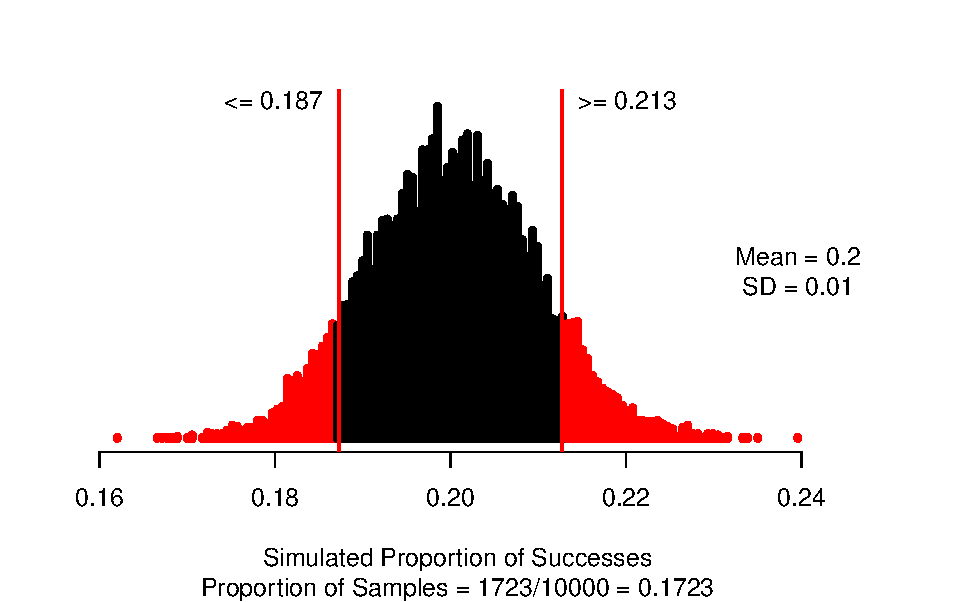
\includegraphics[width=0.7\linewidth]{05-UR-module3_review_files/figure-latex/unnamed-chunk-2-1} \end{center}

\begin{enumerate}
\def\labelenumi{\arabic{enumi}.}
\setcounter{enumi}{6}
\tightlist
\item
  Interpret the p-value in context of the problem.
\end{enumerate}

\vspace{1in}

\begin{enumerate}
\def\labelenumi{\arabic{enumi}.}
\setcounter{enumi}{7}
\tightlist
\item
  How much evidence does the data provide against the null hypothesis?
\end{enumerate}

\begin{center}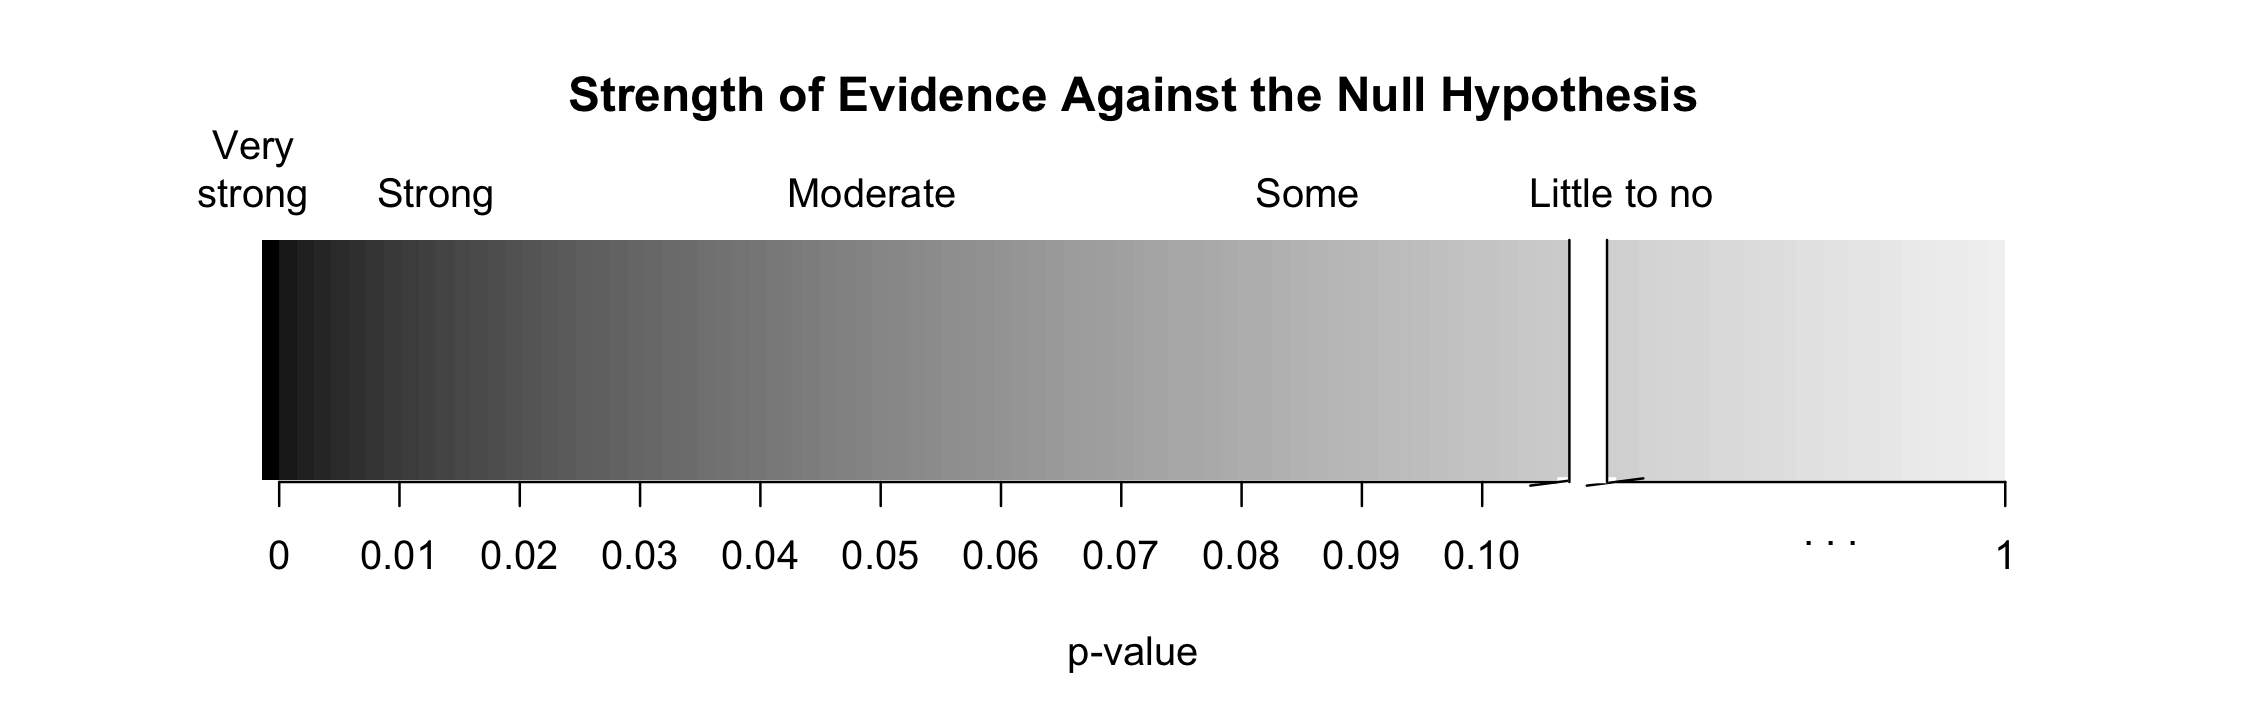
\includegraphics[width=0.9\linewidth]{images/soe_gradient_gray} \end{center}

\vspace{0.2in}

\begin{enumerate}
\def\labelenumi{\arabic{enumi}.}
\setcounter{enumi}{8}
\tightlist
\item
  Write a conclusion to the study in context of the problem.
\end{enumerate}

\vspace{0.8in}

\begin{enumerate}
\def\labelenumi{\arabic{enumi}.}
\setcounter{enumi}{9}
\tightlist
\item
  Would a 95\% confidence interval contain the null value of 0.2? Explain.
\end{enumerate}

\vspace{0.8in}

\begin{enumerate}
\def\labelenumi{\arabic{enumi}.}
\setcounter{enumi}{10}
\tightlist
\item
  What values should be entered for each of the following into the simulation to create the bootstrap distribution of sample proportions to find a 95\% confidence interval?
  \vspace{1mm}
\end{enumerate}

\begin{itemize}
\tightlist
\item
  Sample size:
\end{itemize}

\vspace{.1in}

\begin{itemize}
\tightlist
\item
  Number of successes:
\end{itemize}

\vspace{.1in}

\begin{itemize}
\tightlist
\item
  Number of repetitions:
\end{itemize}

\vspace{.1in}

\begin{itemize}
\tightlist
\item
  Confidence level (as a decimal):
\end{itemize}

\vspace{.1in}

\begin{Shaded}
\begin{Highlighting}[]
\FunctionTok{set.seed}\NormalTok{(}\DecValTok{216}\NormalTok{)}
\FunctionTok{one\_proportion\_bootstrap\_CI}\NormalTok{(}\AttributeTok{sample\_size =} \DecValTok{1753}\NormalTok{, }\CommentTok{\# Sample size}
                    \AttributeTok{number\_successes =} \DecValTok{328}\NormalTok{, }\CommentTok{\# Observed number of successes}
                    \AttributeTok{number\_repetitions =} \DecValTok{10000}\NormalTok{, }\CommentTok{\# Number of bootstrap samples to use}
                    \AttributeTok{confidence\_level =} \FloatTok{0.95}\NormalTok{) }\CommentTok{\# Confidence level as a decimal}
\end{Highlighting}
\end{Shaded}

\begin{center}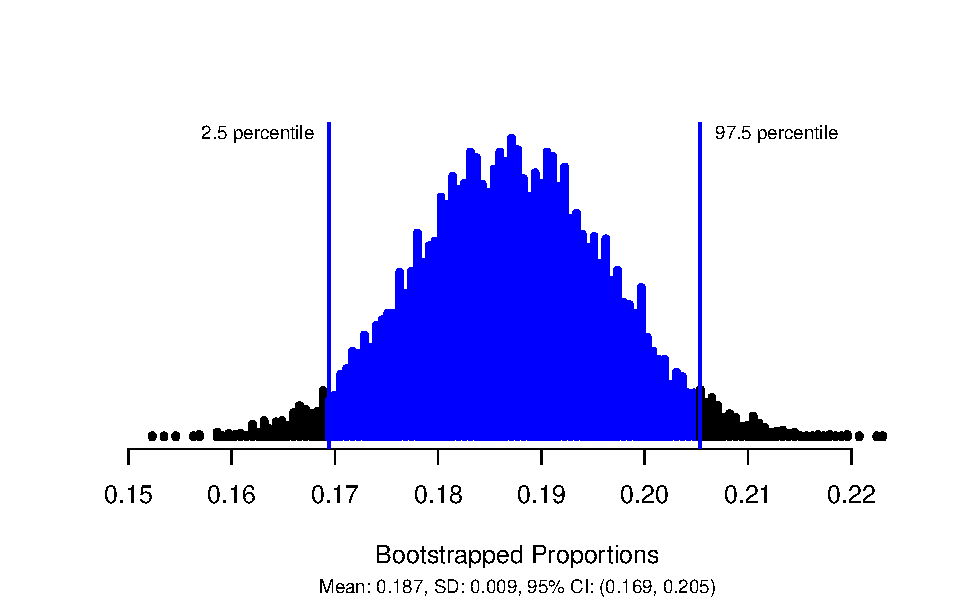
\includegraphics[width=0.7\linewidth]{05-UR-module3_review_files/figure-latex/unnamed-chunk-4-1} \end{center}

\begin{enumerate}
\def\labelenumi{\arabic{enumi}.}
\setcounter{enumi}{11}
\tightlist
\item
  Explain how to use cards to create one bootstrap sample.
\end{enumerate}

\vspace{1in}

\begin{enumerate}
\def\labelenumi{\arabic{enumi}.}
\setcounter{enumi}{12}
\tightlist
\item
  Report the 95\% confidence interval in interval notation.
\end{enumerate}

\vspace{0.2in}

\begin{enumerate}
\def\labelenumi{\arabic{enumi}.}
\setcounter{enumi}{13}
\tightlist
\item
  Interpret the 95\% confidence interval in context of the problem.
\end{enumerate}

\vspace{0.8in}

\newpage

\section{Module 4 Review}\label{module-4-review}

Statistician Jessica Utts has conducted an extensive analysis of Ganzfeld studies that have investigated psychic functioning. Ganzfeld studies involve a ``sender'' and a ``receiver.'' Two people are placed in separate rooms. The sender looks at a ``target'' image on a television screen and attempts to transmit information about the target to the receiver. The receiver is then shown four possible choices or targets, one of which is the correct target and the other three are ``decoys.'' The receiver must choose the one he or she thinks best matches the description transmitted by the sender. If the correct target is chosen by the receiver, the session is a ``hit.'' Otherwise, it is a miss. Utts reported that her analysis considered a total of 2,124 sessions and found a total of 709 ``hits'' (Utts, 2010). Is there evidence of psychic ability?

\begin{enumerate}
\def\labelenumi{\arabic{enumi}.}
\tightlist
\item
  Write the parameter of interest in context of the study.
\end{enumerate}

\vspace{0.6in}

\begin{enumerate}
\def\labelenumi{\arabic{enumi}.}
\setcounter{enumi}{1}
\tightlist
\item
  Calculate the point estimate. Use proper notation.
\end{enumerate}

\vspace{0.3in}

\begin{enumerate}
\def\labelenumi{\arabic{enumi}.}
\setcounter{enumi}{2}
\tightlist
\item
  Write the null hypothesis in words.
\end{enumerate}

\vspace{0.6in}

\begin{enumerate}
\def\labelenumi{\arabic{enumi}.}
\setcounter{enumi}{3}
\tightlist
\item
  Write the alternative hypothesis in notation.
\end{enumerate}

\vspace{0.2in}

A single proportion can be mathematically modeled using the normal distribution if certain conditions are met.

Conditions for the sampling distribution of \(\hat{p}\) to follow an approximate normal distribution.

\begin{itemize}
\item
  Independence: The sample's observations are independent, e.g., are from a simple random sample
\item
  Large enough sample size:

  \begin{itemize}
  \tightlist
  \item
    Success-Failure Condition: There are at least 10 successes and 10 failures in the sample
  \end{itemize}
\end{itemize}

\[n \times \hat{p} \ge 10\] and \[n \times (1-\hat{p}) \ge 10\]

\begin{enumerate}
\def\labelenumi{\arabic{enumi}.}
\setcounter{enumi}{4}
\tightlist
\item
  Are the conditions met to model the data with the Normal distribution?
\end{enumerate}

\vspace{0.6in}

Standardized sample proportion.

The standardized statistic for theory-based methods for one proportion is:

\[Z = \frac{\hat{p}-\pi_0}{SE_0(\hat{p})}\]

Where \[SE_0(\hat{p})=\sqrt\frac{\pi_0\times (1-\pi_0)}{n}\]

\begin{enumerate}
\def\labelenumi{\arabic{enumi}.}
\setcounter{enumi}{5}
\tightlist
\item
  Calculate the null standard error of the sample proportion
\end{enumerate}

\vspace{0.6in}

\begin{enumerate}
\def\labelenumi{\arabic{enumi}.}
\setcounter{enumi}{6}
\tightlist
\item
  Calculate the standardized statistic for the sample proportion.
\end{enumerate}

\vspace{0.4in}

\begin{figure}

{\centering 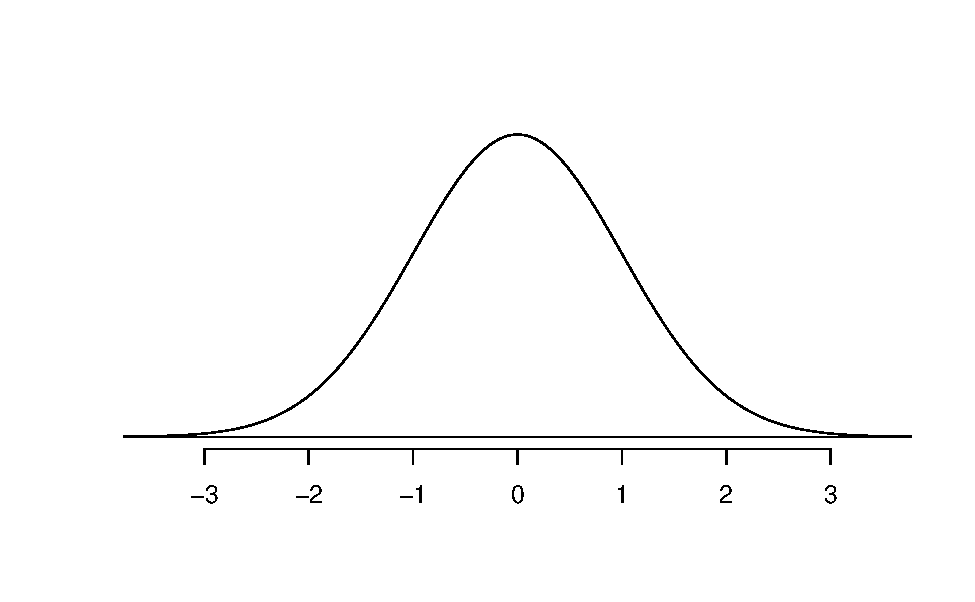
\includegraphics[width=0.5\linewidth]{05-UR-module4_review_files/figure-latex/simpleNormalcurve-1} 

}

\caption{A standard normal curve.}\label{fig:simpleNormalcurve}
\end{figure}

\begin{center}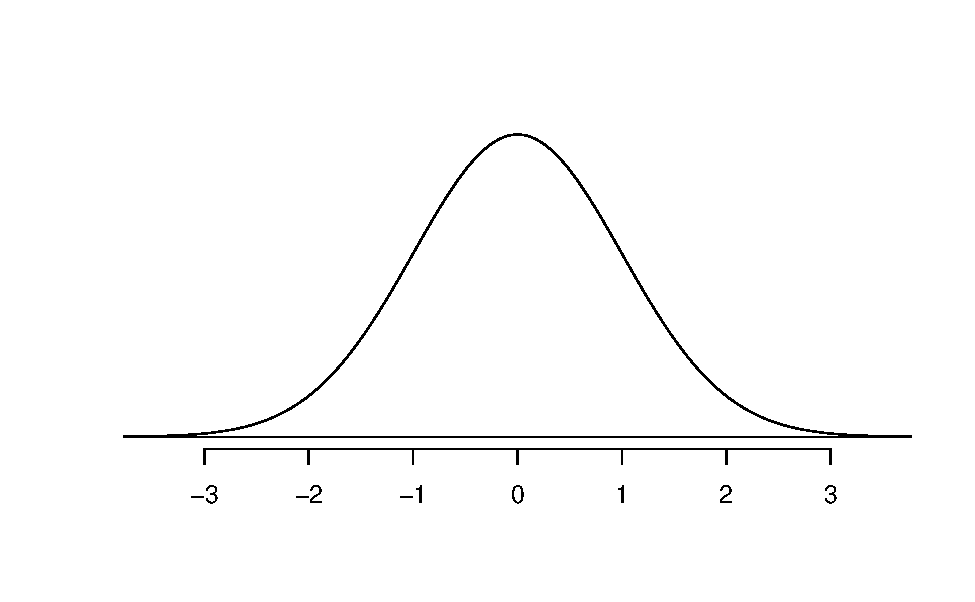
\includegraphics[width=0.5\linewidth]{05-UR-module4_review_files/figure-latex/Normcurve-1} \end{center}

\newpage

\begin{enumerate}
\def\labelenumi{\arabic{enumi}.}
\setcounter{enumi}{7}
\tightlist
\item
  Interpret the standardized statistic in context of the problem.
\end{enumerate}

\vspace{1in}

We will use the \texttt{pnorm()} function in \texttt{R} to find the p-value. The value of the standardized statistic calculated in question 8 is entered into the \texttt{R} code. We used \texttt{lower.tail\ =\ FALSE} to find the p-value so that \texttt{R} will calculate the p-value \emph{greater} than the value of the standardized statistic.

Notes:

\begin{itemize}
\tightlist
\item
  Use \texttt{lower.tail\ =\ TRUE} when doing a left-sided test.
\item
  Use \texttt{lower.tail\ =\ FALSE} when doing a right-sided test.
\item
  To find a two-sided p-value, use a left-sided test for negative Z or a right-sided test for positive Z, then multiply the value found by 2 to get the p-value.
\end{itemize}

\begin{Shaded}
\begin{Highlighting}[]
\FunctionTok{pnorm}\NormalTok{(}\FloatTok{9.333}\NormalTok{, }\CommentTok{\# Enter value of standardized statistic}
      \AttributeTok{m=}\DecValTok{0}\NormalTok{, }\AttributeTok{s=}\DecValTok{1}\NormalTok{, }\CommentTok{\# Using the standard normal mean = 0, sd = 1}
      \AttributeTok{lower.tail=}\ConstantTok{FALSE}\NormalTok{) }\CommentTok{\# Gives a p{-}value greater than the standardized statistic}
\CommentTok{\#\textgreater{} [1] 5.145792e{-}21}
\end{Highlighting}
\end{Shaded}

\begin{enumerate}
\def\labelenumi{\arabic{enumi}.}
\setcounter{enumi}{8}
\tightlist
\item
  Report the value of the p-value.
\end{enumerate}

\vspace{0.1in}

Simulation Method:

\begin{Shaded}
\begin{Highlighting}[]
\FunctionTok{set.seed}\NormalTok{(}\DecValTok{216}\NormalTok{)}
\FunctionTok{one\_proportion\_test}\NormalTok{(}\AttributeTok{probability\_success =} \FloatTok{0.25}\NormalTok{, }\CommentTok{\#Null hypothesis value}
                    \AttributeTok{sample\_size =} \DecValTok{2124}\NormalTok{, }\CommentTok{\#Enter sample size}
                    \AttributeTok{number\_repetitions =} \DecValTok{1000}\NormalTok{, }\CommentTok{\#Enter number of simulations}
                    \AttributeTok{as\_extreme\_as =} \FloatTok{0.334}\NormalTok{, }\CommentTok{\#observed statistic}
                    \AttributeTok{direction =} \StringTok{"greater"}\NormalTok{, }\CommentTok{\#specify direction of alternative hypothesis}
                    \AttributeTok{summary\_measure =} \StringTok{"proportion"}\NormalTok{) }\CommentTok{\#Reporting proportion or number of successes?}
\end{Highlighting}
\end{Shaded}

\begin{center}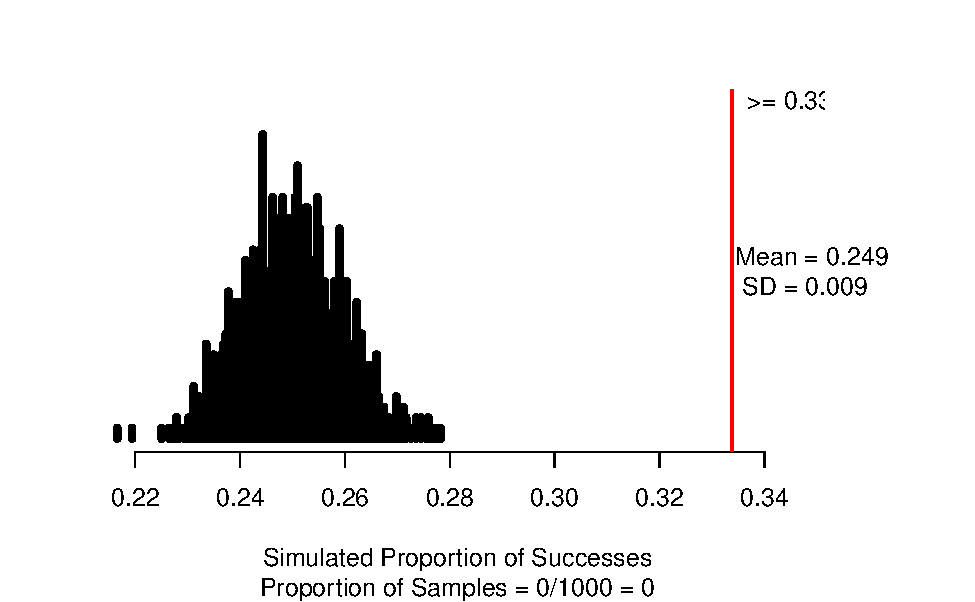
\includegraphics[width=0.8\linewidth]{05-UR-module4_review_files/figure-latex/unnamed-chunk-2-1} \end{center}

\begin{enumerate}
\def\labelenumi{\arabic{enumi}.}
\setcounter{enumi}{9}
\tightlist
\item
  Interpret the p-value in context of the study.
\end{enumerate}

\vspace{0.8in}

Next we will use theory-based methods to estimate the parameter of interest.

To calculate a theory-based 95\% confidence interval for \(\pi\), we will first find the \textbf{standard error} of \(\hat{p}\) by plugging in the value of \(\hat{p}\) for \(\pi\) in \(SD(\hat{p})\):

\[SE(\hat{p}) = \sqrt{\frac{\hat{p}\times(1-\hat{p})}{n}}.\]
Note that we do not include a ``0'' subscript, since we are not assuming a null hypothesis.

\begin{enumerate}
\def\labelenumi{\arabic{enumi}.}
\setcounter{enumi}{10}
\tightlist
\item
  Calculate the standard error of the sample proportion to find a 95\% confidence interval.
\end{enumerate}

\vspace{0.5in}

To find the confidence interval, we will add and subtract the \textbf{margin of error} to the point estimate:

\[\text{point estimate}\pm\text{margin of error}\]
\[\hat{p}\pm z^* SE(\hat{p})\]

The \(z^*\) multiplier is the percentile of a standard normal distribution that corresponds to our confidence level. If our confidence level is 95\%, we find the Z values that encompass the middle 95\% of the standard normal distribution. If 95\% of the standard normal distribution should be in the middle, that leaves 5\% in the tails, or 2.5\% in each tail. The \texttt{qnorm()} function in \texttt{R} will tell us the \(z^*\) value for the desired percentile (in this case, 95\% + 2.5\% = 97.5\% percentile).

\begin{figure}

{\centering 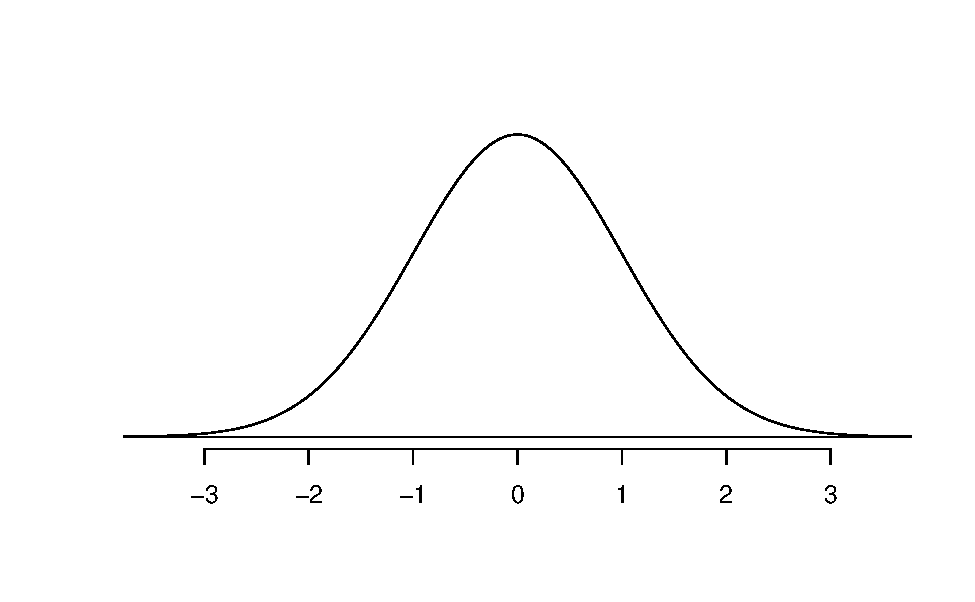
\includegraphics[width=0.5\linewidth]{05-UR-module4_review_files/figure-latex/Ncurve-1} 

}

\caption{A standard normal curve.}\label{fig:Ncurve}
\end{figure}

\begin{Shaded}
\begin{Highlighting}[]
\FunctionTok{qnorm}\NormalTok{(}\FloatTok{0.975}\NormalTok{) }\CommentTok{\# Multiplier for 95\% confidence interval}
\end{Highlighting}
\end{Shaded}

\begin{verbatim}
#> [1] 1.959964
\end{verbatim}

\begin{enumerate}
\def\labelenumi{\arabic{enumi}.}
\setcounter{enumi}{11}
\tightlist
\item
  Calculate the margin of error for a 95\% confidence interval for the true proportion of sessions that will result in a hit.
\end{enumerate}

\vspace{0.6in}

\begin{enumerate}
\def\labelenumi{\arabic{enumi}.}
\setcounter{enumi}{12}
\tightlist
\item
  Calculate the 95\% confidence interval for the true proportion of sessions that will result in a hit.
\end{enumerate}

\vspace{1in}

\newpage

Simulation Methods:

\begin{Shaded}
\begin{Highlighting}[]
\FunctionTok{set.seed}\NormalTok{(}\DecValTok{216}\NormalTok{)}
\FunctionTok{one\_proportion\_bootstrap\_CI}\NormalTok{(}\AttributeTok{sample\_size =} \DecValTok{2124}\NormalTok{, }\CommentTok{\# Sample size}
                    \AttributeTok{number\_successes =} \DecValTok{709}\NormalTok{, }\CommentTok{\# Observed number of successes}
                    \AttributeTok{number\_repetitions =} \DecValTok{10000}\NormalTok{, }\CommentTok{\# Number of bootstrap samples to use}
                    \AttributeTok{confidence\_level =} \FloatTok{0.95}\NormalTok{) }\CommentTok{\# Confidence level as a decimal}
\end{Highlighting}
\end{Shaded}

\begin{center}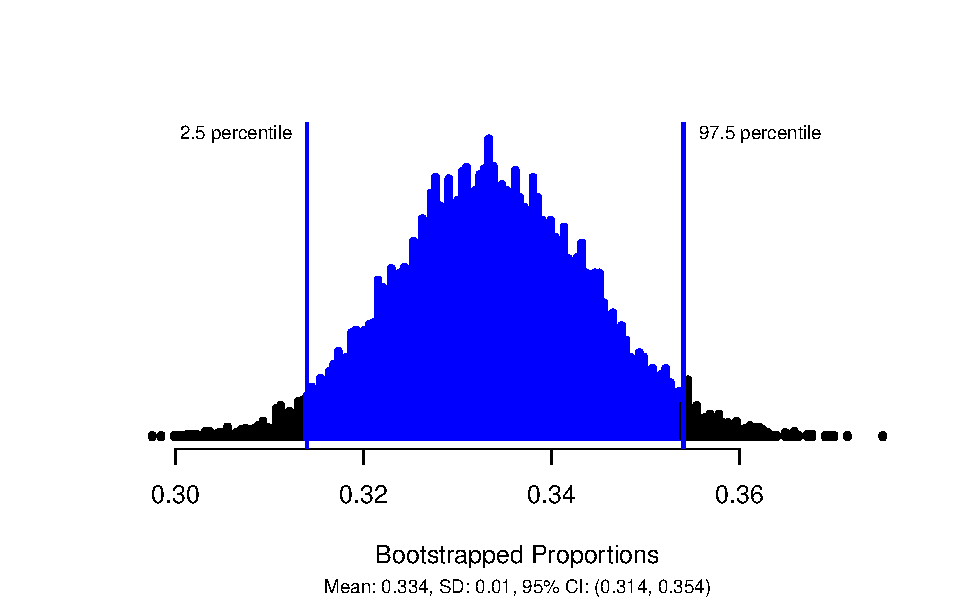
\includegraphics[width=0.8\linewidth]{05-UR-module4_review_files/figure-latex/unnamed-chunk-4-1} \end{center}

\begin{enumerate}
\def\labelenumi{\arabic{enumi}.}
\setcounter{enumi}{13}
\item
  Interpret the 95\% confidence interval in context of the problem.
  \vspace{0.6in}
\item
  Write a conclusion based on the p-value and the 95\% confidence interval.
\end{enumerate}

\vspace{0.6in}

\newpage

\section{Key Topics Exam 1}\label{key-topics-exam-1}

\subsection*{Descriptive statistics and study design}\label{descriptive-statistics-and-study-design}
\addcontentsline{toc}{subsection}{Descriptive statistics and study design}

\begin{enumerate}
\def\labelenumi{\arabic{enumi}.}
\item
  Identify the observational units.
\item
  Identify the types of variables (categorical or quantitative).
\item
  Identify the explanatory variable (if present) and the response variable (roles of variables).
\item
  Identify the appropriate type of graph and summary measure.
\item
  Identify if a given value is a statistic or a parameter. Identify the appropriate notation.
\item
  Identify the study design (observational study or randomized experiment).
\item
  Identify the sampling method and potential types of sampling bias (non-response, response, selection).
\item
  Identify and interpret the summary statistic
\item
  Identify the target population
\item
  Identify the types of sampling bias (response, non-response, selection, none)
\item
  Identify the type(s) of graph(s) that could be used to plot the given variable(s).
\end{enumerate}

\subsection*{Hypothesis testing}\label{hypothesis-testing}
\addcontentsline{toc}{subsection}{Hypothesis testing}

\begin{enumerate}
\def\labelenumi{\arabic{enumi}.}
\setcounter{enumi}{11}
\item
  Write the parameter of interest in context of the problem.
\item
  State the null and alternative hypotheses in both words and notation
\item
  Verify the validity condition is met to use simulation-based methods to find a p-value.
\item
  Verify the validity conditions are met to use theory-based methods to find a p-value from the theoretical distribution.
\item
  In a simulation-based hypothesis test, describe how to create one dot on a dotplot of the null distribution using coins, cards, or spinners.
\item
  Explain where the null distribution is centered and why.
\item
  Describe and illustrate how R calculates the p-value for a simulation-based test.
\item
  Describe and illustrate how R calculates the p-value for a theory-based test.
\item
  Type of theoretical distribution (standard normal distribution or t-distribution with appropriate degrees of freedom) used to model the standardized statistic in a theory-based hypothesis test.
\item
  Calculate and interpret the standard error of the statistic under the null using the correct formula on the Golden ticket.
\item
  Calculate and interpret the appropriate standardized statistic using the correct formula on the Golden ticket.
\item
  Interpret the p-value in context of the study: it is the probability of \_\_\_\_, assuming \_\_\_\_.
\item
  Evaluate the p-value for strength of evidence against the null: how much evidence does the p-value provide against the null?
\item
  Write a conclusion about the research question based on the p-value.
\item
  Describe which features of the study impact the p-value and how.
\end{enumerate}

\subsection{Confidence intervals}\label{confidence-intervals}

\begin{enumerate}
\def\labelenumi{\arabic{enumi}.}
\setcounter{enumi}{26}
\item
  Describe how to simulate one bootstrapped sample using cards.
\item
  Explain where the bootstrap distribution is centered and why.
\item
  Find an appropriate percentile confidence interval using a bootstrap distribution from R output.
\item
  Verify the validity condition is met to use simulation-based methods to find the confidence interval.
\item
  Verify the validity conditions are met to use theory-based methods to calculate a confidence interval.
\item
  Describe and illustrate how the bootstrap distribution is used to find the confidence interval for a given confidence level.
\item
  Describe and illustrate how the standard normal distribution or t-distribution is used to find the multiplier for a given confidence level.
\item
  Calculate and interpret the standard error of the statistic (not assuming the null hypothesis) using the correct formula on the Golden ticket
\item
  Calculate the appropriate margin of error and confidence interval using theory-based methods.
\item
  Interpret the confidence interval in context of the study.
\item
  Based on the interval, what decision can you make about the null hypothesis? Does the confidence interval agree with the results of the hypothesis test? Justify your answer.
\item
  Interpret the confidence level in context of the study. What does ``confidence'' mean?
\item
  Describe which features of the study have an effect on the width of the confidence interval and how.
\end{enumerate}

\newpage

\phantomsection\label{refs}
\begin{CSLReferences}{1}{0}
\bibitem[\citeproctext]{ref-pga}
{``Average Driving Distance and Fairway Accuracy.''} 2008. \href{https://www.pga.com/\%20and\%20https://www.lpga.com/}{https://www.pga.com/ and https://www.lpga.com/}.

\bibitem[\citeproctext]{ref-banton2022}
Banton, et al, S. 2022. {``Jog with Your Dog: Dog Owner Exercise Routines Predict Dog Exercise Routines and Perception of Ideal Body Weight.''} \emph{PLoS ONE} 17(8).

\bibitem[\citeproctext]{ref-bhavsar2022}
Bhavsar, et al, A. 2022. {``Increased Risk of Herpes Zoster in Adults \(\geq\)50 Years Old Diagnosed with COVID-19 in the United States.''} \emph{Open Forum Infectious Diseases} 9(5).

\bibitem[\citeproctext]{ref-islands}
Bulmer, M. n.d. {``Islands in Schools Project.''} \url{https://sites.google.com/site/islandsinschoolsprojectwebsite/home}.

\bibitem[\citeproctext]{ref-bts}
{``Bureau of Transportation Statistics.''} 2019. \url{https://www.bts.gov/}.

\bibitem[\citeproctext]{ref-babies}
{``Child Health and Development Studies.''} n.d. \url{https://www.chdstudies.org/}.

\bibitem[\citeproctext]{ref-darley1973}
Darley, J. M., and C. D. Batson. 1973. {``"From Jerusalem to Jericho": A Study of Situational and Dispositional Variables in Helping Behavior.''} \emph{Journal of Personality and Social Psychology} 27: 100--108.

\bibitem[\citeproctext]{ref-davis2020}
Davis, Smith, A. K. 2020. {``A Poor Substitute for the Real Thing: Captive-Reared Monarch Butterflies Are Weaker, Paler and Have Less Elongated Wings Than Wild Migrants.''} \emph{Biology Letters} 16.

\bibitem[\citeproctext]{ref-doit2015}
Du Toit, et al, G. 2015. {``Randomized Trial of Peanut Consumption in Infants at Risk for Peanut Allergy.''} \emph{New England Journal of Medicine} 372.

\bibitem[\citeproctext]{ref-edmunds2016}
Edmunds, et al, D. 2016. {``Chronic Wasting Disease Drives Population Decline of White-Tailed Deer.''} \emph{PLoS ONE} 11(8).

\bibitem[\citeproctext]{ref-ipeds}
Education Statistics, National Center for. 2018. {``IPEDS.''} \url{https://nces.ed.gov/ipeds/}.

\bibitem[\citeproctext]{ref-gbmarried}
{``Great Britain Married Couples: Great Britain Office of Population Census and Surveys.''} n.d. \url{https://discovery.nationalarchives.gov.uk/details/r/C13351}.

\bibitem[\citeproctext]{ref-zeitler2012}
Group, TODAY Study. 2012. {``\href{https://www.ncbi.nlm.nih.gov/pubmed/22540912}{A Clinical Trial to Maintain Glycemic Control in Youth with Type 2 Diabetes}.''} \emph{New England Journal of Medicine} 366: 2247--56.

\bibitem[\citeproctext]{ref-hamblin2007}
Hamblin, J. K., K. Wynn, and P. Bloom. 2007. {``Social Evaluation by Preverbal Infants.''} \emph{Nature} 450 (6288): 557--59.

\bibitem[\citeproctext]{ref-hirschfelder2018}
Hirschfelder, A., and P. F. Molin. 2018. {``I Is for Ignoble: Stereotyping Native Americans.''} \href{Retrieved\%20from\%20https://www.ferris.edu/HTMLS/news/jimcrow/native/homepage.htm.}{Retrieved from https://www.ferris.edu/HTMLS/news/jimcrow/native/homepage.htm.}

\bibitem[\citeproctext]{ref-hutchison2013}
Hutchison, R. L., and M. A. Hirthler. 2013. {``\href{https://www.ncbi.nlm.nih.gov/pubmed/23932117}{Upper Extremity Injuies in Homer's Iliad}.''} \emph{Journal of Hand Surgery (American Volume)} 38: 1790--93.

\bibitem[\citeproctext]{ref-imdb}
{``{IMDb} Movies Extensive Dataset.''} 2016. \url{https://kaggle.com/stefanoleone992/imdb-extensive-dataset}.

\bibitem[\citeproctext]{ref-kalra2022}
Kalra, et al., Dl. 2022. {``Trustworthiness of Indian Youtubers.''} Kaggle. \url{https://doi.org/10.34740/KAGGLE/DSV/4426566}.

\bibitem[\citeproctext]{ref-keating2021}
Keating, D., N. Ahmed, F. Nirappil, Stanley-Becker I., and L. Bernstein. 2021. {``Coronavirus Infections Dropping Where People Are Vaccinated, Rising Where They Are Not, Post Analysis Finds.''} \emph{Washington Post}. \url{https://www.washingtonpost.com/health/2021/06/14/covid-cases-vaccination-rates/}.

\bibitem[\citeproctext]{ref-laeng2007}
Laeng, Mathisen, B. 2007. {``Why Do Blue-Eyed Men Prefer Women with the Same Eye Color?''} \emph{Behavioral Ecology and Sociobiology} 61(3).

\bibitem[\citeproctext]{ref-levin2000}
Levin, D. T. 2000. {``Race as a Visual Feature: Using Visual Search and Perceptual Discrimination Tasks to Understand Face Categories and the Cross-Race Recognition Deficit.''} \emph{Journal of Experimental Psychology} 129(4).

\bibitem[\citeproctext]{ref-luetkemeier2017}
LUETKEMEIER, et al., M. 2017. {``Skin Tattoos Alter Sweat Rate and Na+ Concentration.''} \emph{Medicine and Science in Sports and Exercise} 49(7).

\bibitem[\citeproctext]{ref-madden2020}
Madden, et al, J. 2020. {``Ready Student One: Exploring the Predictors of Student Learning in Virtual Reality.''} \emph{PLoS ONE} 15(3).

\bibitem[\citeproctext]{ref-miller1956}
Miller, G. A. 1956. {``The Magical Number Seven, Plus or Minus Two: Some Limits on Our Capacity for Processing Information.''} \emph{Psychological Review} 63(2).

\bibitem[\citeproctext]{ref-becentispeech}
Moquin, W., and C. Van Doren. 1973. {``Great Documents in American Indian History.''} Praeger.

\bibitem[\citeproctext]{ref-pew2022}
{``More Americans Are Joining the 'Cashless' Economy.''} 2022. \url{https://www.pewresearch.org/short-reads/2022/10/05/more-americans-are-joining-the-cashless-economy/.}

\bibitem[\citeproctext]{ref-weather}
National Weather Service Corporate Image Web Team. n.d. {``National Weather Service -- {NWS} Billings.''} \url{https://w2.weather.gov/climate/xmacis.php?wfo=byz}.

\bibitem[\citeproctext]{ref-obrien2019}
O'Brien, Lynch, H. D. 2019. {``Crocodylian Head Width Allometry and Phylogenetic Prediction of Body Size in Extinct Crocodyliforms.''} \emph{Integrative Organismal Biology} 1.

\bibitem[\citeproctext]{ref-ocean}
{``Ocean Temperature and Salinity Study.''} n.d. \url{https://calcofi.org/}.

\bibitem[\citeproctext]{ref-WashPost2022}
{``Older People Who Get Covid Are at Increased Risk of Getting Shingles.''} 2022. \url{https://www.washingtonpost.com/health/2022/04/19/shingles-and-covid-over-50/.}

\bibitem[\citeproctext]{ref-physhealth}
{``Physician's Health Study.''} n.d. \url{https://phs.bwh.harvard.edu/}.

\bibitem[\citeproctext]{ref-porath2017}
Porath, Erez, C. 2017. {``Does Rudeness Really Matter? The Effects of Rudeness on Task Performance and Helpfulness.''} \emph{Academy of Management Journal} 50.

\bibitem[\citeproctext]{ref-quinn1999}
Quinn, G. E., C. H. Shin, M. G. Maguire, and R. A. Stone. 1999. {``Myopia and Ambient Lighting at Night.''} \emph{Nature} 399 (6732): 113--14. \url{https://doi.org/10.1038/20094}.

\bibitem[\citeproctext]{ref-ramachandran2007}
Ramachandran, V. 2007. {``3 Clues to Understanding Your Brain.''} \url{https://www.ted.com/talks/vs_ramachandran_3_clues_to_understanding_your_brain}.

\bibitem[\citeproctext]{ref-cdchospitalization}
{``Rates of Laboratory-Confimed COVID-19 Hospitalizations by Vaccination Status.''} 2021. CDC. \url{https://covid.cdc.gov/covid-data-tracker/\#covidnet-hospitalizations-vaccination}.

\bibitem[\citeproctext]{ref-richardson2019}
Richardson, T., and R. T. Gilman. 2019. {``Left-Handedness Is Associated with Greater Fighting Success in Humans.''} \emph{Scientific Reports} 9 (1): 15402. \url{https://doi.org/10.1038/s41598-019-51975-3}.

\bibitem[\citeproctext]{ref-stephens2020}
Stephens, R., and O. Robertson. 2020. {``Swearing as a Response to Pain: Assessing Hypoalgesic Effects of Novel "Swear" Words.''} \emph{Frontiers in Psychology} 11: 643--62.

\bibitem[\citeproctext]{ref-stewart2014}
Stewart, E. H., B. Davis, B. L. Clemans-Taylor, B. Littenberg, C. A. Estrada, and R. M. Centor. 2014. {``Rapid Antigen Group a Streptococcus Test to Diagnose Pharyngitis: A Systematic Review and Meta-Analysis''} 9 (11). \url{https://doi.org/10.1371/journal.pone.0111727}.

\bibitem[\citeproctext]{ref-stroop1935}
Stroop, J. R. 1935. {``Studies of Interference in Serial Verbal Reactions.''} \emph{Journal of Experimental Psychology} 18: 643--62.

\bibitem[\citeproctext]{ref-subach2022}
Subach, et al, A. 2022. {``Foraging Behaviour, Habitat Use and Population Size of the Desert Horned Viper in the Negev Desert.''} \emph{Soc.Open Sci} 9.

\bibitem[\citeproctext]{ref-sulheim2017}
Sulheim, S., A. Ekeland, I. Holme, and R. Bahr. 2017. {``Helmet Use and Risk of Head Injuries in Alpine Skiers and Snowboarders: Changes After an Interval of One Decade''} 51 (1): 44--50. \url{https://doi.org/10.1136/bjsports-2015-095798}.

\bibitem[\citeproctext]{ref-titanic}
{``Titanic.''} n.d. \url{http://www.encyclopedia-titanica.org}.

\bibitem[\citeproctext]{ref-covidvaccinetracker}
{``US COVID-19 Vaccine Tracker: See Your State's Progress.''} 2021. Mayo Clinic. \url{https://www.mayoclinic.org/coronavirus-covid-19/vaccine-tracker}.

\bibitem[\citeproctext]{ref-usepa2020}
US Environmental Protection Agency. n.d. {``Air Data -- Daily Air Quality Tracker.''} \url{https://www.epa.gov/outdoor-air-quality-data/air-data-daily-air-quality-tracker}.

\bibitem[\citeproctext]{ref-wahlstrom2014}
Wahlstrom, et al, K. 2014. {``Examining the Impact of Later School Start Times on the Health and Academic Performance of High School Students: A Multi-Site Study.''} \emph{Center for Applied Research and Educational Improvement}.

\bibitem[\citeproctext]{ref-watson2015}
Watson, et al., N. 2015. {``Recommended Amount of Sleep for a Heathy Adult: A Joint Consensus Statement of the American Academy of Sleep Medicine and Sleep Research Society.''} \emph{Sleep} 38(6).

\bibitem[\citeproctext]{ref-Weiss1988}
Weiss, R. D. 1988. {``Relapse to Cocaine Abuse After Initiating Desipramine Treatment.''} \emph{JAMA} 260(17).

\bibitem[\citeproctext]{ref-navajo2011}
{``Welcome to the Navajo Nation Government: Official Site of the Navajo Nation.''} 2011.\href{\%20Retrieved\%20from\%20https://www.navajo-nsn.gov/.}{Retrieved from https://www.navajo-nsn.gov/.}

\bibitem[\citeproctext]{ref-wilson2016}
Wilson, Woodruff, J. P. 2016. {``Vertebral Adaptations to Large Body Size in Theropod Dinosaurs.''} \emph{PLoS ONE} 11(7).

\end{CSLReferences}

\end{document}
